\section{Further Enhancements}
\label{cha::rsr::enhancements}

Consider an empty rectangle of width $w$ and height $h$ where $w > h$.  After
adding all non-dominated macro edges, each node from the perimeter will have
between $h$ to $2h-1$ neighbours from the opposite side of the rectangle, up to
2 neighbours from the same side of the rectangle and up to 5 other neighbours
from adjacent rectangles.  Such a high branching factor is undesirable as
individual node expansion operations take longer.

In this section we study two branching factor reduction methods.  The first is
an offline technique that prunes nodes from the perimeter of each rectangle.
The second is an online pruning strategy which we apply during individual node
expansion operations.  We discuss both methods in the context of 8-connected
grid maps however they are equally applicable to 4-connected maps.

\subsection{Perimeter Reduction}
\label{cha::rsr::perimeter_reduction}

\begin{figure}[tb]
	\begin{center}
	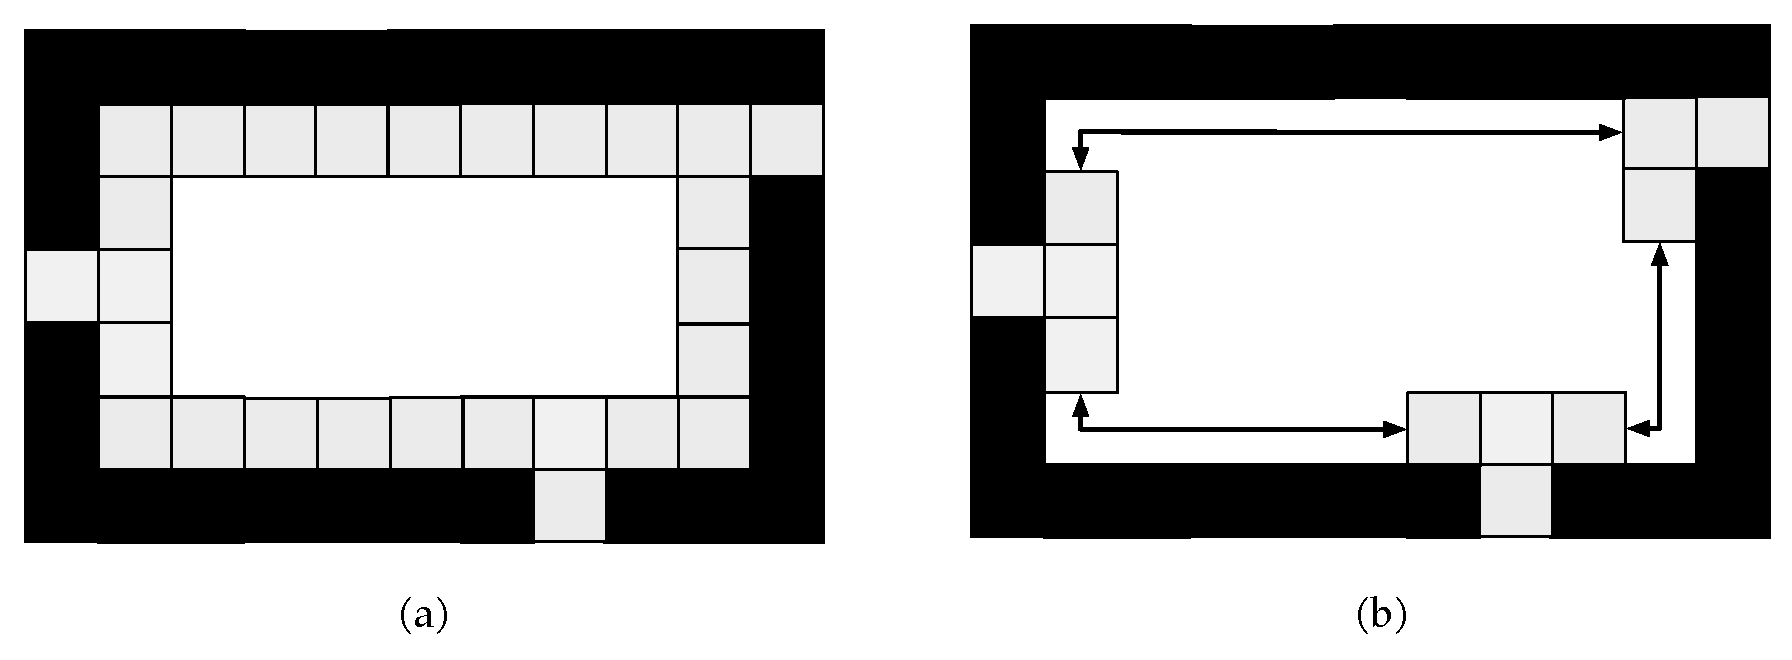
\includegraphics[width=0.95\columnwidth, trim = 10mm 10mm 10mm 0mm]
	{chapter_rsr/diagrams/perimeter_pruning.pdf}
	\end{center}
	\vspace{-3pt}
	\caption[RSR enhancement: perimeter reduction]
    {\small
    (a) From each empty rectangle we prune all nodes which
	have no neighbours in any adjacent rectangle. (b)
	Remaining perimeter nodes are then connected directly.
}
\label{fig::rsr::perimeter_reduction}
\end{figure}

We observe that in both 4-connected and 8-connected maps there are many cases
where nodes on the perimeter of an empty rectangle have no neighbours from any
adjacent rectangle.  Such nodes are adjacent to obstacles and cannot lead into
or out of any empty rectangle.  Figure \ref{fig::rsr::perimeter_reduction}(a)
shows an example.  We propose to prune all such perimeter nodes. To preserve
optimality, we will connect the neighbours of each pruned node directly to
each other.  The weight of each new edge is set appropriately to the octile
distance between the two neighbours\footnote{This operation shares some similarity
to Contraction Hierarchies; a well known and very fast algorithm for finding
shortest paths in road networks. Like RSR, this work creates an abstract
(but multi-level) representation of the graph in which single edges are replaced 
by equivalent-cost ``shortcuts'' (i.e macro-edges).~\cite{geisberger08}}.
Figure~\ref{fig::rsr::perimeter_reduction}(b) shows the result of this
procedure.  As we will see such perimeter reduction can have a dramatic effect
on the average performance of A* on certain types of maps.
\begin{lemma}
Perimeter reduction preserves path optimality.
\end{lemma}
\begin{proof}
Each time we prune a node from the perimeter we add a new edge between
all its neighbours with weight equal to the distance between each pair
of neighbours.  Thus, if a path exists between a pair of nodes before the
application of perimeter reduction it is guaranteed to exist afterward.
Further, the cost of this path is unchanged.
\end{proof}

\subsection{Online Node Pruning}
\label{cha::rsr::online_pruning}

\begin{figure}[bt]
	\begin{center}
	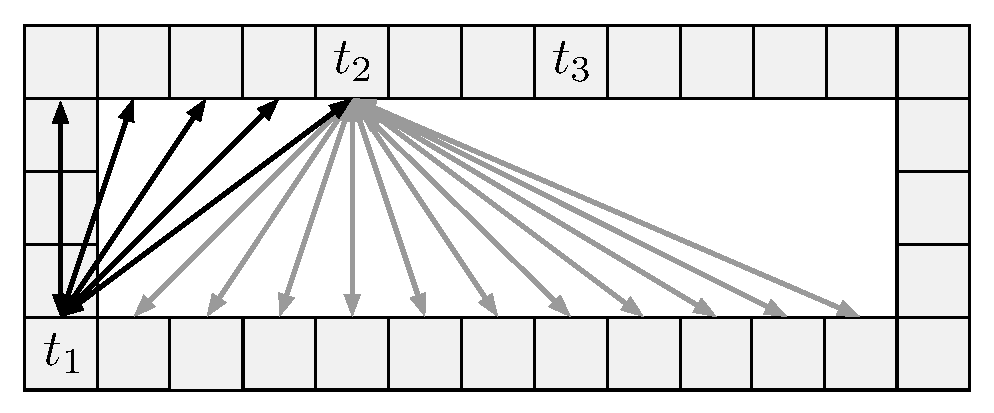
\includegraphics[width=0.5\columnwidth, trim = 10mm 10mm 10mm 0mm]
	{chapter_rsr/diagrams/online_pruning.pdf}
	\end{center}
	\vspace{-3pt}
	\caption[RSR enhancement: online pruning]
    {\small
	Assume that $t_{1}$ is the parent of $t_2$. When $t_2$
	is expanded, there is no need to generate its secondary neighbors
	(nodes connected to $t_2$ by grey edges). These nodes can be reached directly 
	from $t_1$ by a shorter or equal-cost path that does not involve $t_2$.
}
\label{fig::rsr::online_pruning}
\end{figure}

Given a perimeter node $n$, let us partition its macro neighbors 
(connected to $n$ by macro-edges)
on the perimeter into 
\emph{primary neighbours} and \emph{secondary neighbours}.  Secondary neighbours are those
which are located on the opposite side of the perimeter to as compared to $n$
(excluding any corner nodes).  Primary neighbours are all the rest.

When expanding an arbitrary node from the perimeter of a rectangle we observe
that it is not necessary to consider any secondary neighbours if both the node
and its predecessor belong to the same rectangle. Figure \ref{fig::rsr::online_pruning}
shows an example of such a situation; any path to a secondary neighbour
is strictly dominated by an alternative path through the predecessor. 
We apply this observation as follows: {During
node expansion, determine which rectangle the parent of the current node belongs
to.} {If the current node has no parent or the parent belongs to a different
rectangle, then process (i.e., generate) all primary and secondary neighbours.
Otherwise, process only primary neighbours.}

\begin{lemma}
Online node pruning preserves path optimality.
\end{lemma}
\begin{proof}
Let $m$ be a node on the perimeter of a rectangle. Assume that its
parent $p$ belongs to the same rectangle.  Let $n$ be a secondary successor of
$m$.  Recall that $n$ and $m$ are on opposite sides of the rectangle.  We argue
below that passing through $m$ cannot possibly improve the best path between $p$
and $n$.  Therefore, there is no need to consider $(m,n)$ macro-edges when $m$
and $p$ belong to the same rectangle.

There are 4 cases when a node $m$ and its parent $p$ belong to the same
rectangle. In case 1, $p$ is a re-inserted node from the interior of the
rectangle.  Obviously, the path segment $p,m,n$ is sub-optimal, as we zigzag from
$p$ to $m$ on one side of the rectangle and then to $n$ on the opposite side of
the rectangle.  In cases 2, 3, and 4, $p$ and $m$ are on opposite sides, on
orthogonal sides or on the same side of the rectangle. As in case 1, it is
possible to check in each case that taking a detour through $m$ does not improve
the shortest path from $p$ to $n$.
\end{proof}


